\documentclass[a4paper,12pt]{article}
\usepackage[utf8]{inputenc}
\usepackage[english]{babel}
\usepackage{setspace}
\usepackage{lipsum}
\usepackage{listings}
\usepackage{xcolor}
\usepackage{graphicx}
\usepackage{float}
\usepackage{capt-of}
\usepackage{geometry}
\geometry{a4paper, top=3cm, bottom=3cm, left=3cm, right=3cm}


% Konfiguration für den Assembler-Code
\definecolor{mygreen}{rgb}{0,0.6,0}
\definecolor{mygray}{rgb}{0.5,0.5,0.5}
\definecolor{mymauve}{rgb}{0.58,0,0.82}

\lstset{ %
  backgroundcolor=\color{white},
  basicstyle=\ttfamily\footnotesize,
  breaklines=true,
  captionpos=b,
  commentstyle=\color{mygreen},
  keywordstyle=\color{blue},
  stringstyle=\color{mymauve},
  frame=single,
  rulecolor=\color{black},
  language=[x86masm]Assembler
}

\begin{document}

% ---------------------------------------
% Deckblatt
% ---------------------------------------
\thispagestyle{empty}
\vspace*{3cm}
\begin{center}
    \textbf{\LARGE{Lab 2: Clock – HCS12 Interrupts \& I/O}}\\[1cm]
    \textbf{\LARGE{Dokumentation}}\\[3cm]
    \textbf{Tim Jauch}\\[0.5cm]
    \textbf{Ergün Bickici}
\end{center}

\newpage

% ---------------------------------------
% Inhaltsverzeichnis
% ---------------------------------------
\tableofcontents
\newpage

% ---------------------------------------
% Abbildungsverzeichnis
% ---------------------------------------
\listoffigures
\newpage

% ---------------------------------------
% Tabellenverzeichnis
% ---------------------------------------
\listoftables
\newpage

\section{Requirements}
The requirements for the clock and the thermometer are as follows:
The current time should be displayed on the LCD in the format HH:MM:SS and updated every second (hour range: 0–23, minute and second range: 0–59). The LED on Port B.0 should toggle every second. For more details, refer to chapter A.2 in the appendix.
At program start, the time should be initialized to 11:59:30. By briefly pressing button SW2, the clock should switch from Normal Mode to Set Mode. In Set Mode, the user can adjust the hours, minutes, and seconds by pressing buttons SW3, SW4, and SW5. While Set Mode is active, the LED on Port B.7 should be turned on.
In addition to the time, the LCD should also display the temperature (e.g., 25°C). The temperature is measured using a temperature-sensitive resistor (simulated in the lab by a potentiometer) connected to the analog port AD.7. The voltage range is 0–5 V, representing a temperature of –30 to +70°C. Your program must read the analog voltage and convert it into a temperature value in “°C.” The temperature display should also update every second.
The first line of the LCD display should periodically toggle between the names of all group members and the text “© IT SS2025.”.

\newpage
\section{User Interface description}
\subsection{LCD display}
\begin{itemize}
  \item 1st line: Names of all group members or “© IT SS2025” alternating every 10s
  \item 2nd line: 23:55:31 25oC Current time in format HH:MM:SS decimal, left aligned.
  Temperature in degrees Celsius decimal, right aligned. Numbers < 10 shall be displayed
  without leading zeros, no “+” sign for positive values!
\end{itemize}
\subsection{LED display}
\begin{itemize}
  \item LED0: toggles once per second (in Normal Mode and in Set Mode)
  \item LED7: off in Normal Mode, on in Set Mode.
\end{itemize}
\subsection{Operating Buttons}
\begin{itemize}
  \item SW2: Short press to switch to Set Mode, press again to switch back to Normal Mode
  \item SW3: Press to increment the hours (in clock Set Mode only)
  \item SW4: Press to increment the minutes (in clock Set Mode only)
  \item SW5: Press to increment the seconds (in clock Set Mode only)
\end{itemize}

\newpage
\section{Debugging}
Needed to change the value to turn on \textbf{ECT}:
\begin{lstlisting}
TIMER_ON equ $80 ; tscr1 value to turn ECT on (value turn on)
\end{lstlisting}
Needed to change value for \textbf{AND} and \textbf{XOR} operation to set the timer prescaler to 128,
which equals a timer driver frequency of 187500 Hz:
\begin{lstlisting}
ldab TSCR2
andb #$80
orab #7
stab TSCR2
\end{lstlisting}
\newpage
\section{Data Dictionary}
\begin{table}[h!]
\centering
\begin{tabular}{|l|l|l|l|}
\hline
\textbf{Module} & \textbf{Variable} & \textbf{C-like datatype} & \textbf{Purpose} \\ \hline
clock.c, main.c & seconds & unsigned char & counting up seconds \\ \hline
clock.c, main.c & minutes & unsigned char & counting up minutes \\ \hline
clock.c, main.c & hours & unsigned char & counting up hours \\ \hline
main.c, constant.h & SELECT12HOURS & unsigned char & switch between 12/24h model \\ \hline
\end{tabular}
\caption{Module variables and their purpose}
\end{table}
\newpage
\section{Module Overview}

\begin{figure}[H]
    \centering
    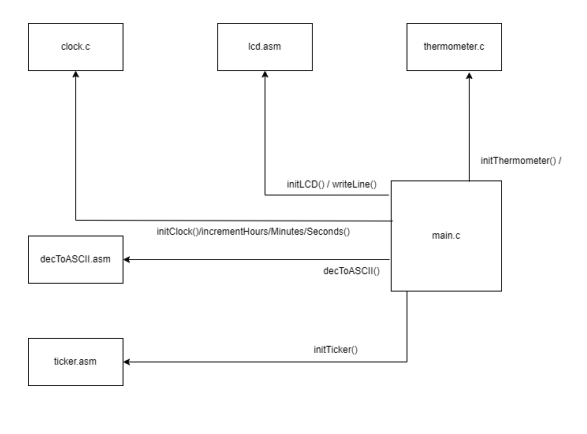
\includegraphics[width=1\textwidth]{diagrams/moduleOverview.png}
    \caption{Module Overview}
    \label{fig:MainModuleOverview}
\end{figure}

\newpage
\section{Interface Descriptions of All Subroutines}

\subsection{main.c}

\begin{description}
    \item[decToASCII\_Wrapper] Wrapper function for \texttt{decToASCII}.
    \begin{itemize}
        \item \textbf{Parameters:} \texttt{char*} pointer to the destination string; \texttt{int} number to convert.
        \item \textbf{Return:} -
    \end{itemize}
    
    \item[WriteLine\_Wrapper] Wrapper function for \texttt{writeLine}.
    \begin{itemize}
        \item \textbf{Parameters:} \texttt{char*} pointer to LCD print location; \texttt{int} LCD line definition.
        \item \textbf{Return:} -
    \end{itemize}
    
    \item[initLED\_C] Initializes the output port for LEDs and LCD (called once).
    \begin{itemize}
        \item \textbf{Parameters:} -
        \item \textbf{Return:} -
    \end{itemize}
    
    \item[toggleLED\_C] Switches LED state.
    \begin{itemize}
        \item \textbf{Parameters:} \texttt{char} bitmask to toggle LEDs.
        \item \textbf{Return:} -
    \end{itemize}
    
    \item[incrementCounter] Advances to the next entry in the array of strings for LCD line 0.
    \begin{itemize}
        \item \textbf{Parameters:} \texttt{unsigned char*} pointer; \texttt{unsigned char} max value.
        \item \textbf{Return:} -
    \end{itemize}
    
    \item[isButtonPressed] Checks if a button is pressed.
    \begin{itemize}
        \item \textbf{Parameters:} \texttt{char} button to check.
        \item \textbf{Return:} \texttt{char} button state (on/off).
    \end{itemize}
    
    \item[WriteLine2\_C] Prepares time/temperature data for LCD display.
    \begin{itemize}
        \item \textbf{Parameters:} -
        \item \textbf{Return:} -
    \end{itemize}
\end{description}

\subsection{ticker.asm}

\begin{description}
    \item[initLCD] Initializes the ticker (called once).
    \begin{itemize}
        \item \textbf{Parameters:} -
        \item \textbf{Return:} -
        \item \textbf{Registers:} Unchanged upon return.
    \end{itemize}
    
    \item[isrECT4] Interrupt service routine triggered by the timer ticker every 10\,ms.
    \begin{itemize}
        \item \textbf{Parameters:} -
        \item \textbf{Return:} -
        \item \textbf{Registers:} Unchanged upon return.
    \end{itemize}
\end{description}

\subsection{decToASCII.asm}

\begin{description}
    \item[decToASCII] Converts a given decimal value (time) to ASCII (called before displaying time).
    \begin{itemize}
        \item \textbf{Parameters:} -
        \item \textbf{Return:} -
        \item \textbf{Registers:} Unchanged upon return.
    \end{itemize}
\end{description}

\subsection{clock.c}

\begin{description}
    \item[initClock] Initializes global time variables (called once).
    \begin{itemize}
        \item \textbf{Parameters:} -
        \item \textbf{Return:} -
    \end{itemize}
    
    \item[incrementHours] Increments the hours.
    \begin{itemize}
        \item \textbf{Parameters:} -
        \item \textbf{Return:} -
    \end{itemize}
    
    \item[incrementMinutes] Increments the minutes.
    \begin{itemize}
        \item \textbf{Parameters:} -
        \item \textbf{Return:} -
    \end{itemize}
    
    \item[tickClock] Calls \texttt{incrementSeconds} with a clock event.
    \begin{itemize}
        \item \textbf{Parameters:} -
        \item \textbf{Return:} -
    \end{itemize}
\end{description}

\subsection{thermometer.c}

\begin{description}
    \item[interrupt service] Measures the current temperature (triggered by interrupt vector 22).
    \begin{itemize}
        \item \textbf{Parameters:} -
        \item \textbf{Return:} -
    \end{itemize}
    
    \item[initThermometer] Initializes the analog input (called once).
    \begin{itemize}
        \item \textbf{Parameters:} -
        \item \textbf{Return:} -
    \end{itemize}
    
    \item[convertTemperature] Converts the analog value to degrees Celsius.
    \begin{itemize}
        \item \textbf{Parameters:} -
        \item \textbf{Return:} -
    \end{itemize}
\end{description}
\newpage
\section{Flow charts}
\subsection{Main}
\subsection{Thermometer}
\begin{figure}[H]
    \centering
    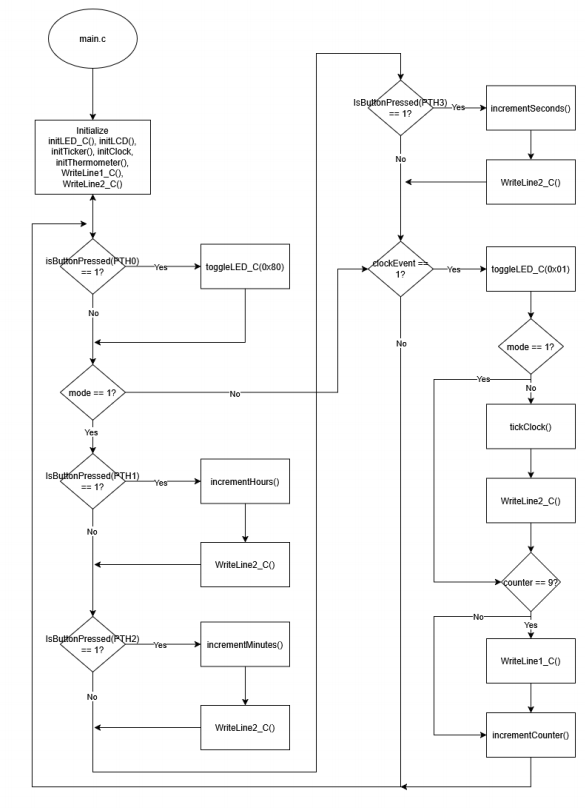
\includegraphics[width=0.9\textwidth]{diagrams/main(2).png}
    \caption{Main}
    \label{fig:Main}
\end{figure}

\newpage

\subsection{Thermometer}
\begin{figure}[H]
    \centering
    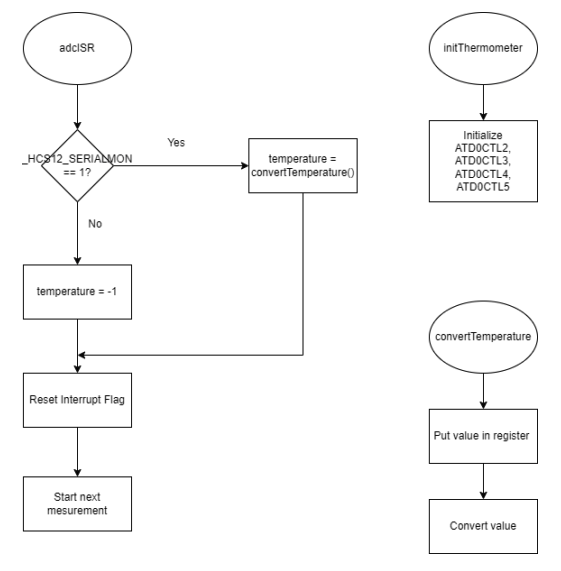
\includegraphics[width=1\textwidth]{diagrams/thermometer.png}
    \caption{Thermometer}
    \label{fig:Thermometer}
\end{figure}

\newpage

\subsection{Ticker}
\begin{figure}[H]
    \centering
    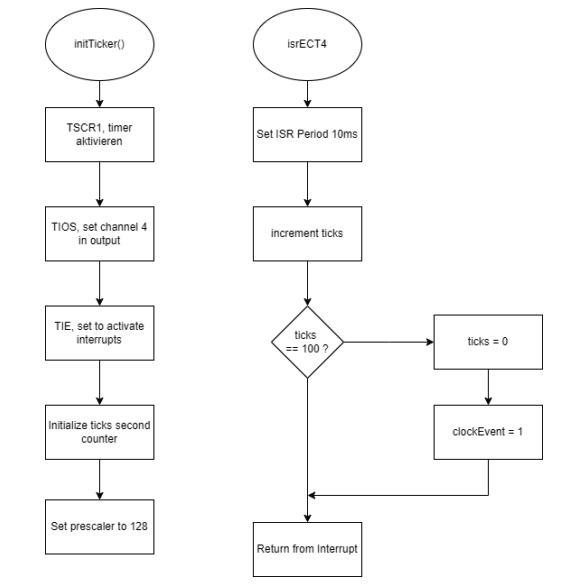
\includegraphics[width=1\textwidth]{diagrams/ticker.png}
    \caption{Ticker}
    \label{fig:Ticker}
\end{figure}

\subsection{Clock}
\begin{figure}[H]
    \centering
    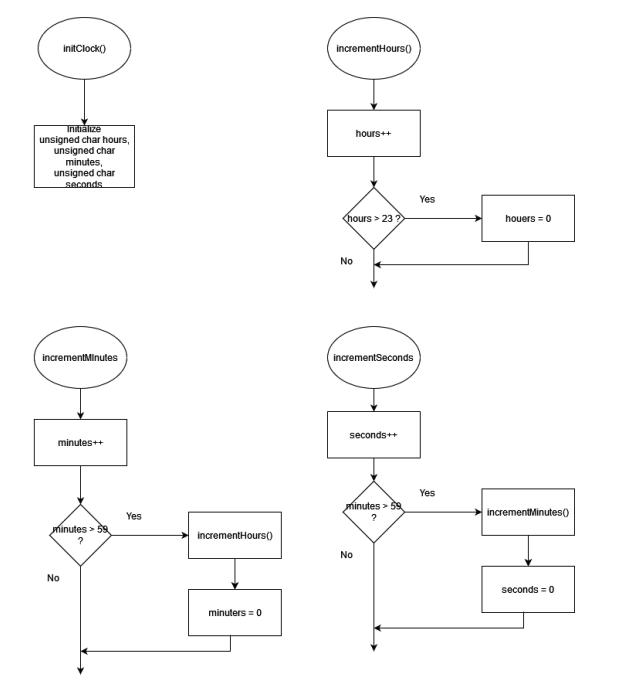
\includegraphics[width=1\textwidth]{diagrams/clock.png}
    \caption{Clock}
    \label{fig:Clock}
\end{figure}

\subsection{DecToASCII}
\begin{figure}[H]
    \centering
    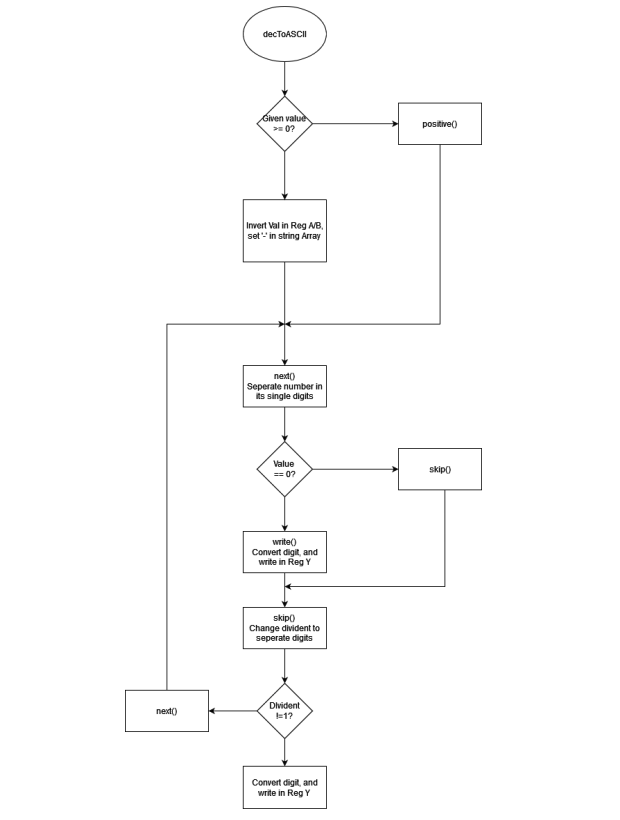
\includegraphics[width=1\textwidth]{diagrams/decToASCII.png}
    \caption{DecToASCII}
    \label{fig:DecToASCII}
\end{figure}

\end{document}
